\section{Design}

FlashMatrix is a matrix-oriented programming framework for general data analysis.
It supports both sparse matrix operations and dense matrix operations. This work
mainly focuses on dense matrices and scales dense matrix operations beyond
memory capacity by utilizing fast I/O devices, such as solid-state drives (SSDs),
in a non-uniform memory architecture (NUMA). The implementation and optimization
of sparse matrix multiplication is described in \cite{SEM_SpMM}.
FlashMatrix uses R as its main programming interface and executes R code
automatically in parallel and out of core.

Figure \ref{fig:arch} shows the architecture of FlashMatrix. The core of
FlashMatrix provides a small number of generalized matrix operators (GenOps)
to simplify the implementation and improve expressiveness of
the framework. The optimizer in FlashMatrix aggressively merges operations to
reduce CPU cache misses and I/O accesses and achieve better parallelization.
FlashMatrix stores large matrices on SSDs through SAFS \cite{safs},
a user-space filesystem for a large SSD array, to fully utilize high I/O
throughput of SSDs and deploys a set of I/O optimizations to improve
its sequential I/O throughput \cite{SEM_SpMM}.

\begin{figure}
\centering
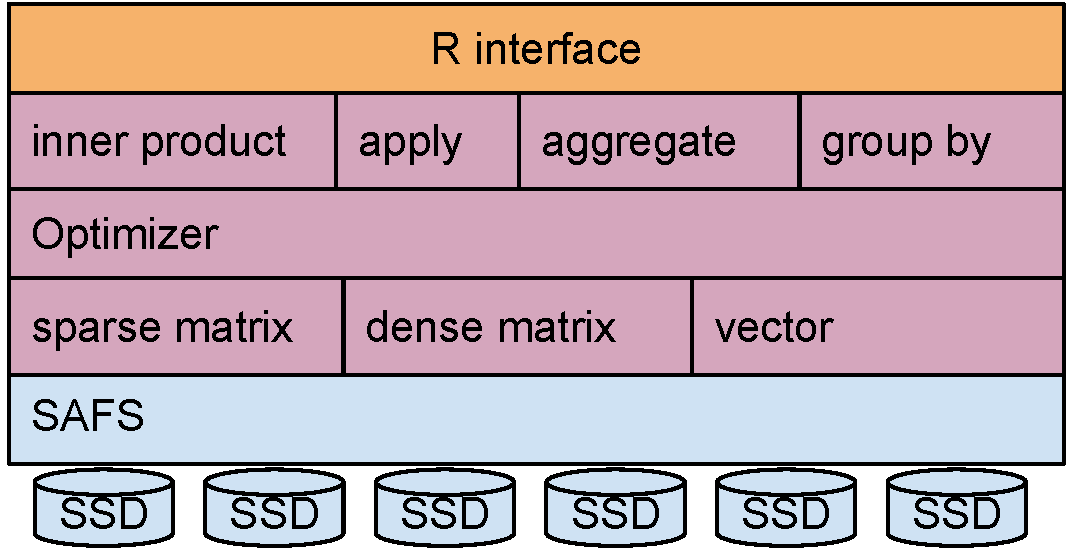
\includegraphics[scale=0.3]{FlashMatrix_figs/architecture.pdf}
\caption{The architecture of FlashMatrix.}
\label{fig:arch}
\end{figure}

\subsection{Dense matrices}
Dense matrices are the main data types in FlashMatrix. A vector is stored
as a one-column dense matrix. In FlashMatrix, a dense matrix can be stored
physically in memory or on SSDs or represented virtually by a sequence of
computation. FlashMatrix specifically optimizes for tall-and-skinny matrices
and short-and-wide matrices, and views tall matrices and wide matrices
as groups of tall-and-skinny matrices and short-and-wide matrices, respectively.

%\begin{figure}
%	\centering
%	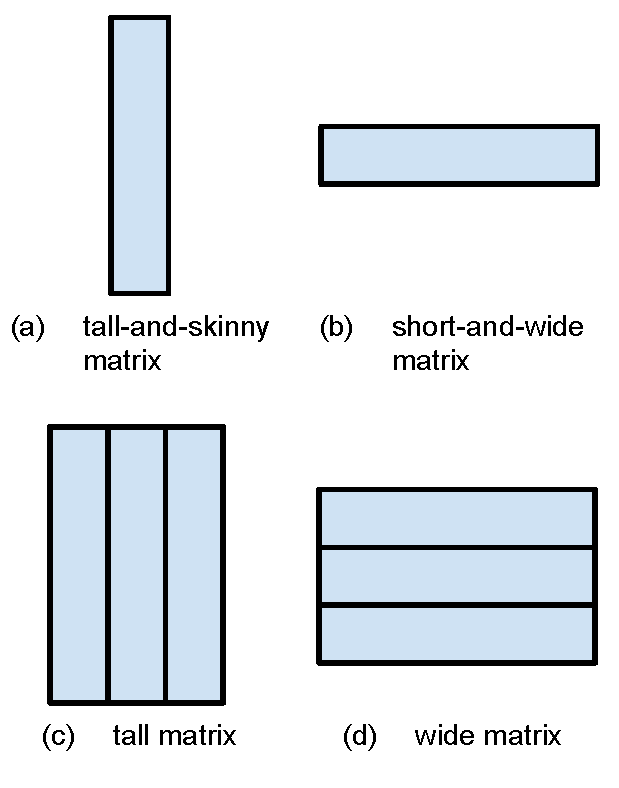
\includegraphics[scale=0.5]{FlashMatrix_figs/matrix.pdf}
%	\caption{Dense matrices of different shapes.}
%	\label{fig:mat}
%\end{figure}

%A matrix has two identifiers: the \textit{matrix identifier} that indicates
%the matrix itself and the \textit{matrix data identifier} that indicates
%the data in the matrix. When a matrix is cloned or transposed, the new matrix
%has a different \textit{matrix identifier} but shares the same
%\textit{matrix data identifier} with the original matrix.

\subsubsection{Tall-and-skinny matrices} \label{sec:tas_mat}

FlashMatrix optimizes for tall-and-skinny (TAS) dense matrices due to their
frequent occurrence in data analysis. In this field, many data matrices contain
a large number of samples with a relatively few features, so
data matrices are usually tall and skinny. If a data matrix has many
features, the first step is often dimension reduction \cite{Jain00}, which
results in a TAS matrix. FlashMatrix specifically optimizes for TAS dense
matrices with tens of columns or fewer.

FlashMatrix supports row-major and column-major matrix layout (Figure
\ref{fig:tas_mat}). As such, we avoid data copy for common matrix operations
such as matrix transpose. FlashMatrix optimizes matrix operations for both
data layouts. Each GenOp has its own preferred matrix layout and determines
the layout of an output matrix based on the input matrices.

\begin{figure}
	\centering
	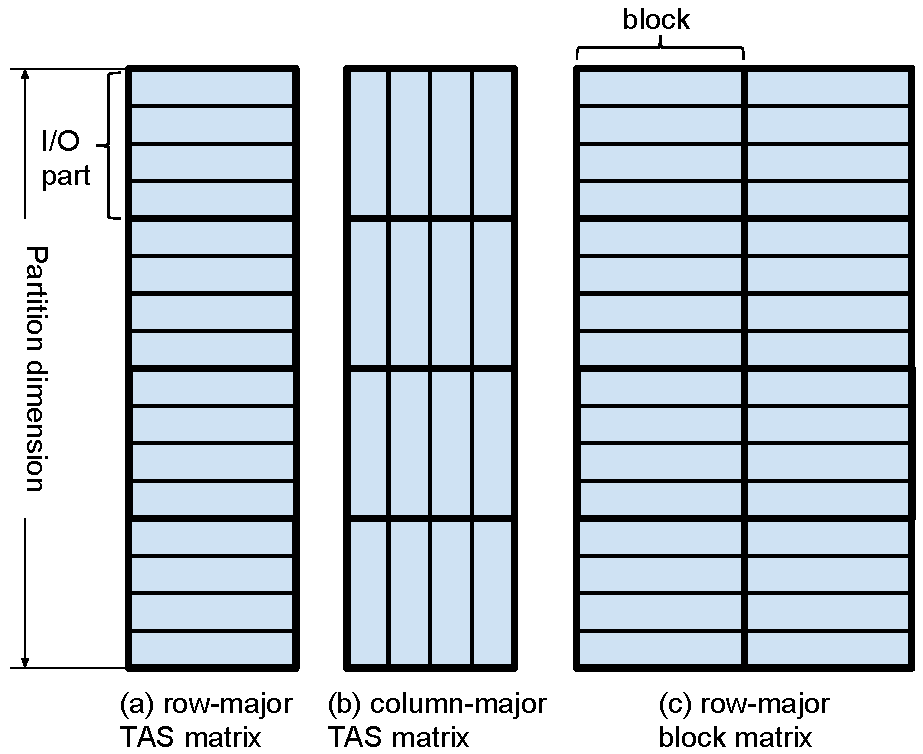
\includegraphics[scale=0.5]{FlashMatrix_figs/dense_matrix2.pdf}
	\caption{The format of a tall-and-skinny dense matrix.}
	\label{fig:tas_mat}
\end{figure}

FlashMatrix uses two-level horizontal partitioning on TAS matrices for
efficient data access to SSDs and main memory (Figure \ref{fig:tas_mat}).
FlashMatrix partitions both in-memory and
external-memory TAS matrices horizontally into I/O-level partitions.
All elements in an I/O-level partition are stored contiguously regardless
of the data layout in the matrix. For an in-memory matrix, the partition
size determines the size of contiguous memory required in memory allocation
(see Section \ref{sec:mem}). For an external-memory matrix, the partition
size determines an I/O size, usually on the order of megabytes, because each
I/O access reads an entire I/O-level partition. The number of rows in
an I/O-level partition is always $2^i$. This produces column-major TAS
matrices whose data are well aligned in memory to help CPU vectorization.
For an in-memory TAS matrix, FlashMatrix maps I/O-level partitions to NUMA
nodes to achieve data locality and full utilization of memory bandwidth.
We map I/O-level partitions of different vectors/matrices involved in
computation to the same NUMA node to reduce remote memory access.
We further split an I/O-level partition
horizontally into CPU-level partitions for computation. We use a small
CPU-level partition (on the order of kilobytes) so that it fits in CPU
L1/L2 cache to reduce CPU cache misses when evaluating a sequence of matrix
operations (Section \ref{sec:lazy_eval}). FlashMatrix determines the number
of rows in a CPU-level partition based on the number of columns in a matrix.

\subsubsection{Virtual matrices} \label{virt_mat}
In many cases, we do not need to store the data of a matrix physically. Instead,
we compute and generate its data on the fly. \textit{Virtual matrices} store
computation and potentially the reference
to some other matrices required by computation. A simple example is a matrix
with all elements having the same value. For such a matrix, we only need to store
a single value and construct its matrix partitions during computation.

\textit{Virtual matrices} are essential for lazy evaluation (Section
\ref{sec:lazy_eval}). All GenOps may output \textit{virtual matrices} that
represent computation results by storing only the computation of GenOps
and the references to input matrices. This strategy is
essential for both in-memory and external-memory optimizations to improve
performance. It significantly reduces data access to memory and SSDs as well as
memory allocation overhead for creating new matrices.

\subsubsection{Cached matrix}
Memory cache is necessary for external-memory matrices on a machine with
substantial memory.
Even though SSDs have substantial I/O performance, they are still
an order of magnitude slower than DRAM. Unfortunately, we cannot rely on
the page cache in SAFS \cite{SA-cache} to buffer some portion of a dense matrix
because streaming an entire matrix to memory evicts existing data in the page
cache and generates zero cache hits. Therefore, FlashMatrix allows users to
explicitly cache part of a dense matrix.

We store a matrix cache as an in-memory dense matrix.
To effectively cache data in a dense matrix, we store a tall matrix in
column-major and cache the first few columns; we store a wide matrix in row-major
and cache the first few rows. As such, when computation requests an I/O-level
partition of a matrix, we only need to issue a single I/O request to read
the remaining columns or rows to reconstruct the I/O-level partition.

We use a write-through policy for the matrix cache. As such, even when part of
a dense matrix is cached, we keep a complete copy of the dense matrix on SSDs.
The write-through policy overlaps computation and I/O when
a dense matrix is created, and avoids I/O latency when removing the cache.

\subsubsection{A group of dense matrices} \label{sec:mat_group}
FlashMatrix represents a tall matrix with a group of
tall-and-skinny matrices and a wide matrix with a group of short-and-wide
matrices. We construct a special \textit{virtual matrix} to represent
a group of dense matrices. To take advantage of the optimizations on matrix
operations on TAS matrices, we decompose a matrix operation on a group of
matrices into operations on individual matrices in the group (Section
\ref{sec:group_op}).
Coupled with the two-level partitioning on TAS matrices, this strategy enables
2D-partitioning on a dense matrix and each partition fits in main memory
or CPU cache.

% TODO
%A group of matrices should be stored in a single SAFS file to reduce the number
%of SAFS files.

%append an element to a vector can be implemented as physically appending the element
%to the vector. The result vector becomes the new vector, and the original vector
%becomes the sub-vector of the new vector.

\subsubsection{Memory management} \label{sec:mem}
Creating in-memory matrices requires large memory allocations, which are
expensive operations in Linux because Linux uses \textit{mmap} to allocate
large memory and relies on page faults to populate the memory. Frequent page
faults prevent computation from fully utilizing CPUs in a large parallel
machine and cause significant performance degradation. The functional
programming interface of FlashMatrix leads to more frequent memory allocation,
because each matrix operation generates a new matrix. 
FlashMatrix manages large memory allocation itself to reduce overhead.

\begin{figure}
	\centering
	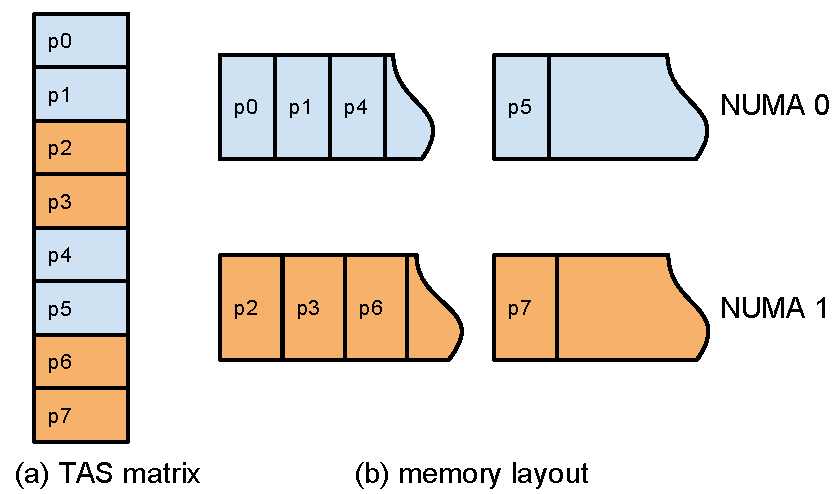
\includegraphics[scale=0.5]{FlashMatrix_figs/matrix_mem.pdf}
	\caption{Memory layout of a tall-and-skinny dense matrix.}
	\label{fig:mat_mem}
\end{figure}

FlashMatrix stores an in-memory matrix in fixed-size memory chunks and
recycles memory chunks to reduce memory allocation overhead (Figure
\ref{fig:mat_mem}). FlashMatrix requires only an I/O-level partition to
be stored in contiguous memory. As long as a memory chunk is sufficient
to store an I/O-level partition, FlashMatrix can store a matrix in a set
of fixed-size memory chunks. The size of a memory chunk is a global parameter
and is the same for all matrices. As such, FlashMatrix reuses memory chunks
allocated for matrices of different shapes. 
%In practice, the memory chunk size
%may not be divisible by an I/O-level partition size. Therefore, the 
We choose the memory chunk
size to be much larger than the I/O-level partition size to increase
memory utilization. We use 64MB as the default memory chunk size.


\subsection{Programming interface}

FlashMatrix provides a matrix-oriented functional programming interface.
The main interface is a small set of GenOps that take matrices and some
element functions (EleFuns) as input and output new matrices that store
computation results. EleFuns define computation on individual elements
in input matrices. We implement both GenOps and EleFuns with C++ and provides
a large set of built-in EleFuns. FlashMatrix
exposes GenOps and the built-in EleFuns in its R interface
and reimplements many functions from the R \textit{base} package with GenOps.

The R interface provides many functions to support varieties of data analysis
algorithms. We categorize the functions into three classes.
\begin{itemize}
	\item The generalized matrix operators (GenOps), listed in Table
		\ref{tbl:genops}.
	\item Utility functions include functions that construct FlashMatrix vectors
		and matrices; functions that convert between FlashMatrix objects and R
		objects; functions that transform the shape of a matrix; functions that
		provide additional control on computation and data storage in FlashMatrix.
		Examples are shown in Table \ref{tbl:utility}.
	\item R matrix computation functions implemented with GenOps. Examples
		are shown in Table \ref{tbl:Rfuns}.
\end{itemize}

\begin{table}
\begin{center}
\footnotesize
\begin{tabular}{|l|l|l|}
\hline
GenOp & Description \\
\hline
$C=fm.inner.prod(A, B, f1, f2)$ & $t=f1(A_{i,k}, B_{k,j})$,
\\ & $C_{i,j}=f2(t, C_{i,j})$,
\\ & over all $k$ \\
\hline
$C=fm.sapply(A, f)$ & $C_{i,j}=f(A_{i,j})$ \\
\hline
$C=fm.mapply(A, B, f)$ & $C_{i,j}=f(A_{i,j}, B_{i,j})$ \\
\hline
$C=fm.mapply.row(A, B, f)$ & $C_{i,j}=f(A_{i,j}, B_j)$ \\
\hline
$C=fm.mapply.col(A, B, f)$ & $C_{i,j}=f(A_{i,j}, B_i)$ \\
\hline
$c=fm.agg(A, f)$ & $c=f(A_{i,j}, c)$, over all $i$, $j$ \\
\hline
$C=fm.agg.row(A, f)$ & $C_i=f(A_{i,j}, C_i)$, over all $j$ \\
\hline
$C=fm.agg.col(A, f)$ & $C_j=f(A_{i,j}, C_j)$, over all $i$ \\
\hline
%$C=fm.groupby(A, f)$ & $C_k=f(A_{i,j}, C_k)$, where $k$ \\
$C=fm.groupby.row(A, B, f)$ & $C_{k,j}=f(A_{i,j}, C_{k,j})$,\\ & where $B_i=k$, over all $i$ \\
\hline
$C=fm.groupby.col(A, B, f)$ & $C_{i,k}=f(A_{i,j}, C_{i,k})$,\\ & where $B_j=k$, over all $j$ \\
\hline
\end{tabular}
\normalsize
\end{center}
\caption{The list of generalized matrix operators (GenOps) in FlashMatrix.
$A$, $B$ and $C$ are matrices, and $c$ is a scalar.}
\label{tbl:genops}
\end{table}

\begin{table}
\begin{center}
\footnotesize
\begin{tabular}{|l|l|l|}
\hline
Class & Function & Description \\
\hline
\multirow{4}{*}{Create} & $fm.rep.int$ & Create a vector of a repeated value \\
& $fm.seq.int$ & Create a vector of sequence numbers \\
& $fm.runif.matrix$ & Create a uniformly random matrix  \\
& $fm.rnorm.matrix$ & Create a random matrix under \\ & & a normal distribution \\
\hline
\multirow{2}{*}{Convert} & $fm.conv.FM2R$ & Convert a FM matrix to an R matrix \\
& $fm.conv.R2FM$ & Convert an R matrix to a FM matrix \\
\hline
\multirow{3}{*}{Reshape} & $t$ & Matrix transpose \\
& $fm.rbind$ & Bind matrices by rows \\
& $fm.cbind$ & Bind matrices by columns \\
\hline
\multirow{4}{*}{Control} & $fm.conv.layout$ & Convert the data layout of a matrix \\
& $fm.set.mate.level$ & Set the materialization level of \\ & & a \textit{virtual matrix} \\
& $fm.materialize$ & Materialize a \textit{virtual matrix} \\
& $fm.conv.store$ & Move a matrix to a specified \\ & & storage \\
\hline
\end{tabular}
\normalsize
\end{center}
\caption{Some of the utility functions in FlashMatrix.}
\label{tbl:utility}
\end{table}

\begin{table}
\begin{center}
\footnotesize
\begin{tabular}{|l|l|l|}
\hline
Class & Function & Description \\
\hline
\multirow{10}{*}{Element-wise} & $C=A+B$ & $C_{i,j}=A_{i,j} + B_{i,j}$ \\
& $C=A-B$ & $C_{i,j}=A_{i,j} - B_{i,j}$ \\
& $C=A*B$ & $C_{i,j}=A_{i,j} * B_{i,j}$ \\
& $C=A/B$ & $C_{i,j}=A_{i,j} / B_{i,j}$ \\
& $C=pmin(A,B)$ & $C_{i,j}=pmin(A_{i,j}, B_{i,j})$ \\
& $C=pmax(A,B)$ & $C_{i,j}=pmax(A_{i,j}, B_{i,j})$ \\
& $C=sqrt(A)$ & $C_{i,j}=sqrt(A_{i,j})$ \\
& $C=abs(A)$ & $C_{i,j}=abs(A_{i,j})$ \\
& $C=exp(A)$ & $C_{i,j}=exp(A_{i,j})$ \\
\hline
\multirow{5}{*}{Aggregate} & $c=sum(A)$ & $c=\sum\limits_{i=1}^{n} \sum\limits_{j=1}^{p}A_{i,j}$ \\
& $C=rowSums(A)$ & $C_i=\sum\limits_{j=1}^{p} A_{i,j}$ \\
& $C=colSums(A)$ & $C_j=\sum\limits_{i=1}^{n} A_{i,j}$ \\
& $c=any(A)$ & true if any element is true \\
& $c=all(A)$ & true if all elements are true \\
\hline
\multirow{1}{*}{multiply} & $\%*\%$ & matrix multiplication \\
\hline
\end{tabular}
\normalsize
\end{center}
\caption{Some of the R functions implemented with GenOps.}
\label{tbl:Rfuns}
\end{table}

\begin{figure}[t]
\begin{minted}[mathescape,
		fontsize=\scriptsize,
		frame=single,
]{R}
# X is the data matrix
# C is the cluster centers from the previous iteration.
kmeans.iter <- function(X, C)
{
	# Compute the pair-wise distance between a data
	# point and a center.
	D <- fm.inner.prod(X, t(C), "euclidean", "+")
	# Find the closest center to a data point.
	I <- fm.agg.row(D, "which.min")
	# Count the number of data points in each cluster.
	one <- fm.rep.int(1, nrow(I))
	CNT <- fm.groupby.row(one, I, "+")
	# Compute the new centers.
	C <- fm.groupby.row(X, I, "+")
	C <- fm.mapply.row(C, CNT, "/")
	list(C=C, I=I)
}
\end{minted}
\vspace{-5pt}
\caption{The R code of computing an iteration of k-means using GenOps.}
\label{fig:kmeans}
\end{figure}

Figure \ref{fig:kmeans} shows an example of computing an iteration of k-means
\cite{kmeans} using GenOps. It first uses \textit{fm.inner.prod} to
compute the Euclidean distance between every data point and every cluster center,
and outputs a matrix with each row representing the distances from a data
point to every cluster center. It uses \textit{fm.agg.row} to find the closest
cluster for each data point and the output matrix represents how data points
are assigned to clusters. It then uses \textit{fm.groupby.row} to count
the number of data points in each cluster and compute the mean of each cluster.

%\subsection{SAFS}

%SAFS \cite{safs} is a user-space filesystem for a high-speed SSD array in
%a NUMA machine. It is implemented as
%a library and runs in the address space of its application. It is deployed
%on top of the Linux native filesystem. SAFS was originally designed for
%optimizing small I/O accesses. However, FlashMatrix accesses data in matrices
%sequentially and
%generates much fewer but much larger I/O. Therefore, we provide additional
%optimizations to maximize sequential I/O throughput from a large SSD array.

%The first optimization is to enable polling for I/O to reduce thread context
%switches. On a high-speed SSD array, the latency caused by a thread context
%switch becomes noticeable under a sequential I/O workload and it becomes
%critical to avoid thread
%context switch to gain I/O performance. If the computation in application
%threads does not saturate CPU, SAFS will put the application threads into
%sleep while they are waiting for I/O. This results in many thread context
%switches and underutilization of both CPU and SSDs. To saturate I/O,
%an application thread issues asynchronous I/O to SAFS and poll for I/O
%completion after completing all computation available to it. Polling avoids
%a thread from being switched out during I/O access and effectively maximizes
%I/O throughput of a high-speed SSD array.

%To better support access to many files simultaneously, SAFS stripes data in
%a file across SSDs with a different striping order for each file. Due to
%the sequential I/O workload, FlashMatrix stripes data across SSDs with a large
%block size, on the order of megabytes, to increase I/O throughput and reduce
%write amplification on SSDs \cite{Tang15}. Such a large block size may cause
%storage skew for small files on a large SSD array if every file stripes data
%in the same order. Using the same striping order also causes skew in I/O access.
%Therefore, SAFS generates a random striping order for each file to evenly
%distribute I/O among SSDs. SAFS stores the striping order with a file for
%future data retrieval.

%When accessing a file sequentially from SSDs, we maintain a set of memory buffers
%for I/O access to reduce the overhead of memory allocation.
%We use large I/O to increase I/O throughput. As such, we need to allocate
%a large memory buffer for I/O access.
%The operating system usually allocates a large memory buffer with \textit{mmap()}
%and populates the buffer with physical pages when it is used. It is
%computationally expensive to populate
%large memory buffers frequently. When accessing high-throughput I/O devices,
%such overhead can cause substantial performance loss. Therefore, we keep a set
%of memory buffers allocated previously and reuse them for new I/O requests.

\subsection{Efficient generalized operations}
FlashMatrix provides efficient implementations of a small number of
generialized matrix operations (GenOps) to achieve both generality and
efficiency. For generality, FlashMatrix allows users to pass functions to
GenOps to define actual matrix computation. For efficiency, FlashMatrix
requires the functions passed to GenOps to be vectorized.

\subsubsection{Generalized matrix operations} \label{sec:genop}
FlashMatrix provides only four GenOps on matrices: \textit{inner product},
\textit{apply}, \textit{aggregation} and \textit{groupby} (Table
\ref{tbl:genops}). Each operator represents a data access pattern and
accepts some element functions as additional
arguments that define computation on individual elements in matrices (Section
\ref{sec:vef}).

\textit{Inner product} is a generalized matrix multiplication (\textit{fm.inner.prod}).
It replaces multiplication and addition in matrix multiplication with two functions.
We define many operations with \textit{inner product}. For example, we use it
to compute various pair-wise distances, such as Euclidean distance and Hamming
distance, between data points. For dense matrices, we mainly focus on optimizing
two cases: \textit{inner product} of a wide matrix and a tall matrix and
\textit{inner product} of a tall matrix and a small matrix. It is impractical to
materialize \textit{inner product} of a large tall matrix and a large wide matrix
owing to space complexity. This holds for all matrix algebra frameworks.
%Common
%practice transforms computation that requires this form of inner product to
%the other two forms to reduce space complexity \cite{}.
%Even though we can implement matrix multiplication with inner product,
When evaluating an \textit{inner product} expression, FlashMatrix uses the BLAS
implementation of matrix multiplication for floating-point matrices.
This achieves the speed and precision required by
numeric libraries, such as eigensolvers \cite{anasazi, flasheigen}.

\textit{Apply} is a generalized form of element-wise operations and has
multiple variants. The simplest variant (\textit{fm.sapply}) is
an element-wise unary operation. We use it to implement many unary
operations such as negation, square root or element type casting
on a matrix. The second variant (\textit{fm.mapply}) is an
element-wise binary operation. We use it to implement many binary
matrix operations such as matrix addition and subtraction. The third
(\textit{fm.mapply.row}) and the fourth variants (\textit{fm.mapply.col}) perform element-wise
binary operations on the input vector with every row or column of the input
matrix and output a matrix of the same shape as the input matrix.

\textit{Aggregation} takes multiple elements and outputs a single element.
It has three variants on a matrix. The first variant (\textit{fm.agg})
aggregates over all elements on a matrix, e.g., matrix summation. The second
(\textit{fm.agg.row}) and the third variants (\textit{fm.agg.col})
compute aggregation over each individual row or column. \textit{rowSums}
and \textit{colSums} in R are examples.

Similarly, \textit{Groupby} on a matrix has two variants.
%The first variant
%(\textit{fm.groupby}) groups elements of a matrix based on the element values
%and performs aggregation on each group of elements.
The first variant (\textit{fm.groupby.row}) groups rows and the second variant
(\textit{fm.groupby.col}) groups columns of a matrix based on a vector of
categorical values and performs aggregation on the rows or
columns associated with the same categorical value. Matrix \textit{groupby}
is used in classification and clustering algorithms that compute
aggregation on the data points in a class or in a cluster.

\subsubsection{Vectorized element functions} \label{sec:vef}
Invoking a function on each element individually would
result in significant function call overheads. Instead, all of
the GenOps take vectorized element functions (VEleFuns) that operate on
a vector of elements instead of an individual element. By transforming
the operations on individual elements to the ones on a vector, we amortize
the overhead of function calls significantly.

We balance the amortization of function call overhead and CPU cache misses.
To reduce latency of accessing data in VEleFuns,
the input data has to be small enough to fit in the CPU L1 cache. On the
other hand, passing a longer vector to a VEleFun amortizes the overhead of
function calls more aggressively. We use 128 as the maximum length of
the input vector of a VEleFun. %Futher increasing the length does not have
%noticeable performance improvement.

We have three types of VEleFuns to support the GenOps in FlashMatrix. Each VEleFun
type may have multiple forms to allow GenOps to transform operations to
increase the length of an input vector to a VEleFun and reduce function call
overhead.
\begin{itemize}
	\item A \textit{unary} VEleFun (\textit{uVEleFun}) takes a vector
		as input and outputs a vector of the same length.
	\item A \textit{binary} VEleFun has three forms: the first form (\textit{bVEleFun1}) 
    takes two vectors of the same length and outputs
		a vector of the same length as the input vectors; the second form (\textit{bVEleFun2}) 
    takes a vector as the left argument and a scalar
		as the right argument and outputs a vector with the same length as
		the input vector; the third form (\textit{bVEleFun3}) takes a scalar
		as the left argument and a vector as the right argument and outputs
		a vector. The second and third forms support non-commutative binary
		operations such as division and subtraction.
	\item An \textit{aggregation} VEleFun consists of two functions:
		\textit{aggregate} and \textit{combine}. Both functions may have two
		forms: the first one (\textit{aVEleFun1}) takes a vector and
		outputs a scalar; the second one (\textit{aVEleFun2}) takes
		two vectors of the same length and outputs a vector. For many
		aggregation VEleFuns such as summation, \textit{aggregate} and
		\textit{combine} are the same and have both \textit{aVEleFun1} and
		\textit{aVEleFun2} forms. For some aggregation such as \textit{count},
		\textit{aggregate} and \textit{combine} are different.
\end{itemize}

FlashMatrix provides many commonly used VEleFuns that wrap basic operations
built in many programming languages and libraries. For example,
FlashMatrix provides arithmetic operations (\textit{addition} and
\textit{subtraction}), relational operations (\textit{equal to} and
\textit{less than}), logical operations (\textit{logical AND} and
\textit{logical OR}), as well as commonly used math functions (\textit{absolute
value} and \textit{square root}). FlashMatrix also provides a set of VEleFuns to
cast primitive element types.

For each basic operation, FlashMatrix provides multiple VEleFun
implementations to support different element types. To reduce the number
of binary VEleFun implementations, FlashMatrix only provides the ones that take
two input arguments of the same type. If a GenOp gets two matrices with different
element types, it first casts the element type of one matrix to match
the other. %Type casting follows the usual arithmetic conversions \cite{}
%commonly seen in many programming languages.
Type casting operations are
implemented with \textit{fm.sapply} and are performed lazily.

FlashMatrix allows programmers to extend the framework by registering new VEleFuns.
Like built-in VEleFuns, a new VEleFun needs to provide multiple
implementations to support different element types; based on the type of
the VEleFun, it may need to provide different forms as described above.
FlashMatrix currently requires a VEleFun to be implemented with C/C++.

We use CPU vector instructions such as AVX \cite{avx} to accelerate
the computation in a VEleFun. The current implementation of FlashMatrix heavily
relies on auto-vectorization of a compiler, such as GCC, to vectorize
computaion. FlashMatrix provides hints and
transforms code to help auto-vectorization. For example, a VEleFun in FlashMatrix
frequently operates on vectors with data aligned in memory and of
the length defined at compile time, so we inform the compiler of the data alignment
and the vector length. Some compilers do not automatically vectorize
aggregation operations well. In this case, we manually create a small vector of reduction
variables, flatten the loop and transform the original aggregation operation
into aggregation onto the vector of reduction variables to help auto-vectorization.

\subsubsection{Implementation of GenOps with VEleFun}

GenOps invoke VEleFuns on the elements of CPU-level partitions intelligently
to increase the length of vectors passed and to reduce the overhead of
function calls. Different GenOps choose different
forms of VEleFuns based on the data layout and the shape of the input matrices.

Some GenOps invoke VEleFuns on the elements of matrices efficiently regardless of
data layout and matrix shape.
For example, \textit{fm.sapply} and \textit{fm.mapply} only require
the input matrices and the output matrix to have the same data layout. For tall
column-major matrices and wide row-major matrices, each CPU-level partition has
long columns and long rows, respectively. These GenOps invoke a VEleFun
on the long columns and rows. For tall row-major matrices and wide column-major
matrices, all rows and columns in a CPU-level partition are stored in a single
piece of memory. These GenOps invoke a VEleFun only once on all
elements in a partition. %A similar strategy is applicable to \textit{agg}.

Most of the GenOps require a matrix with a specific data layout to reduce
function call overhead.
Many of the GenOps favor the column-major order for a tall-and-skinny matrix
and the row-major order for a short-and-wide matrix. These data layouts increase
the length of a vector passed to a VEleFun and align data in memory. For example,
the column-major order ensures that each column in a partition of a tall matrix
is aligned in memory, regardless of the number of columns in the matrix. A GenOp,
such as inner product, converts the data layout of a CPU-level partition to
the preferred layout if an input matrix does not have the preferred layout.
%Because a CPU-level partition fits in the CPU cache, data layout conversion
%does not increase data access to main memory. 

Given a matrix with the preferred data layout, a GenOp selects different forms
of a VEleFun automatically based on the shape of the input matrix. For example,
for a tall column-major matrix, \textit{fm.mapply.col} invokes the \textit{bVEleFun1}
form of the binary VEleFun on a column from the input matrix and the input vector;
for a wide row-major matrix, \textit{fm.mapply.col} invokes the \textit{bVEleFun2}
form on a row from the input matrix and an element from the vector. We apply
the similar strategy to other GenOps. When applying \textit{inner product}
on a tall column-major matrix, FlashMatrix uses the \textit{bVEleFun2} form of
the first VEleFun to computes the outer product of a column from the left matrix
and a row from the right matrix, and uses the \textit{aVEleFun2} of the second VEleFun
to compute the final result. Because \textit{inner product} operates on
a CPU-level partition, all intermediate results in the computation reside
in CPU cache. Inner product on a wide matrix and a tall matrix invokes the
\textit{bVEleFun1} form of the first VEleFun on a row from the left matrix and a column
from the right matrix, and invokes the \textit{aVEleFun1} form of the second VEleFun
on the output from the first VEleFun to compute an element in the output matrix for
the input partitions.

%Both \textit{agg\_row} and \textit{agg\_col} work better on the preferred data
%layout if the aggregation VEleFun has the same \textit{aggregate} and \textit{combine}
%function with both \textit{aVEleFun1} and \textit{aVEleFun2} forms. For these aggregation
%VEleFuns, we can transform \textit{agg\_row} on a column-major matrix to applying
%\textit{aVEleFun2} to columns of a partition. Similar transformation is applied
%to \textit{agg\_col} on a row-major matrix.

%Inner product chooses different forms of VEleFuns for input matrices with different
%shapes. The first UDF of inner product is a binary UDF and the second one is an
%aggregation UDF. For the sake of efficiency, inner product requires the second
%UDF to have the same \textit{aggregate} and \textit{combine} function with both
%\textit{aVEleFun1} and \textit{aVEleFun2} forms.

%Unlike other GenOps, \textit{groupby\_row} and \textit{groupby\_col} are the only
%GenOps that do not favor the column-major order for a tall-and-skinny matrix and
%the row-major order for a short-and-wide matrix. \textit{groupby\_row} sorts
%rows in a partition based on the categorical values associated with each row
%and apply the aggregation VEleFun on rows directly.

\subsubsection{Implementation of GenOps on a group of matrices} \label{sec:group_op}

When applying a GenOp on a group of matrices (Section \ref{sec:mat_group}),
we decompose the computation into multiple GenOps and apply them to individual
matrices in the group if the GenOp supports decomposition. Decomposing computation
to individual matrices reduces memory copies and increases CPU cache hits.
For the GenOps that cannot be decomposed, we combine the individual matrices
on the fly and apply the GenOps on the combined matrix directly.

We apply some of the GenOps to individual matrices directly without
transformation. For example,
\textit{fm.sapply} and \textit{fm.agg} run on individual matrices directly regardless
of the shape and data layout of the matrices. Other GenOps may be applied
to individual matrices directly if the input matrices have certain shape. For
example, we apply \textit{fm.mapply.col} and \textit{fm.agg.col} to individual
matrices in a group of tall matrices directly.  Similarly, we apply
\textit{fm.mapply.row} and \textit{fm.agg.row} to
individual matrices in a group of wide matrices directly. %\textit{mapply}
%requires the matrices in the two input matrix groups to have the same shape.
%\textit{Groupby\_row} on a \textit{tall matrix group} can be decomposed and
%applied to individual matrices; \textit{groupby\_col} on a \textit{wide matrix group}
%can be decomposed in a similar fashion.

Applying other GenOps to a group of matrices requires transformation. If an aggregation
VEleFun provides a \textit{combine} function, applying \textit{fm.agg.row} to a group of
tall matrices is transformed into two steps: apply the \textit{aggregate} function on
each row of individual matrices and apply the \textit{combine} function on the partial
aggregation results. When applying \textit{fm.mapply.row} to a group of tall matrices,
we break the input vector into parts to match the number of columns in the individual
matrices in the group and apply \textit{fm.mapply.row} to individual matrices
separately. We apply the same strategies to \textit{fm.agg.col} and
\textit{fm.mapply.col} on a group of wide matrices. 

%FlashMatrix decomposes inner product on a matrix group in favor of minimizing
%the amount of data written to SSDs (Figure \ref{fig:inner_prod}).
%For \textit{inner\_prod\_tall}, we first partition the right matrix vertically
%and compute the inner product of the left matrix with each vertical partition
%of the right matrix, which outputs
%part of a final output matrix. The number of vertical partitions determines
%the number of runs required to complete the inner product on the group of matrices.
%If the left matrix is stored on SSDs, the number of vertical partitions on
%the right matrix determines the number of times that the left matrix is read
%from SSDs. The vertical
%partition size also determines the output matrix size in each run and affect
%the memory size. As such, we need to select the vertical partition size of
%the right matrix to balance I/O and memory consumption. We horizontally partition
%each vertical partition of the right matrix to further decompose the inner
%product. We construct a directed acyclic graph (DAG) to evalute the inner
%product lazily (Section \ref{sec:lazy_eval}). Similarly, we partition the right
%matrix and make a similar choice to balance I/O and memory consumption for
%\textit{inner\_prod\_wide}. We also construct a DAG and lazily evaluate
%the computation.

%\begin{figure}
%\centering
%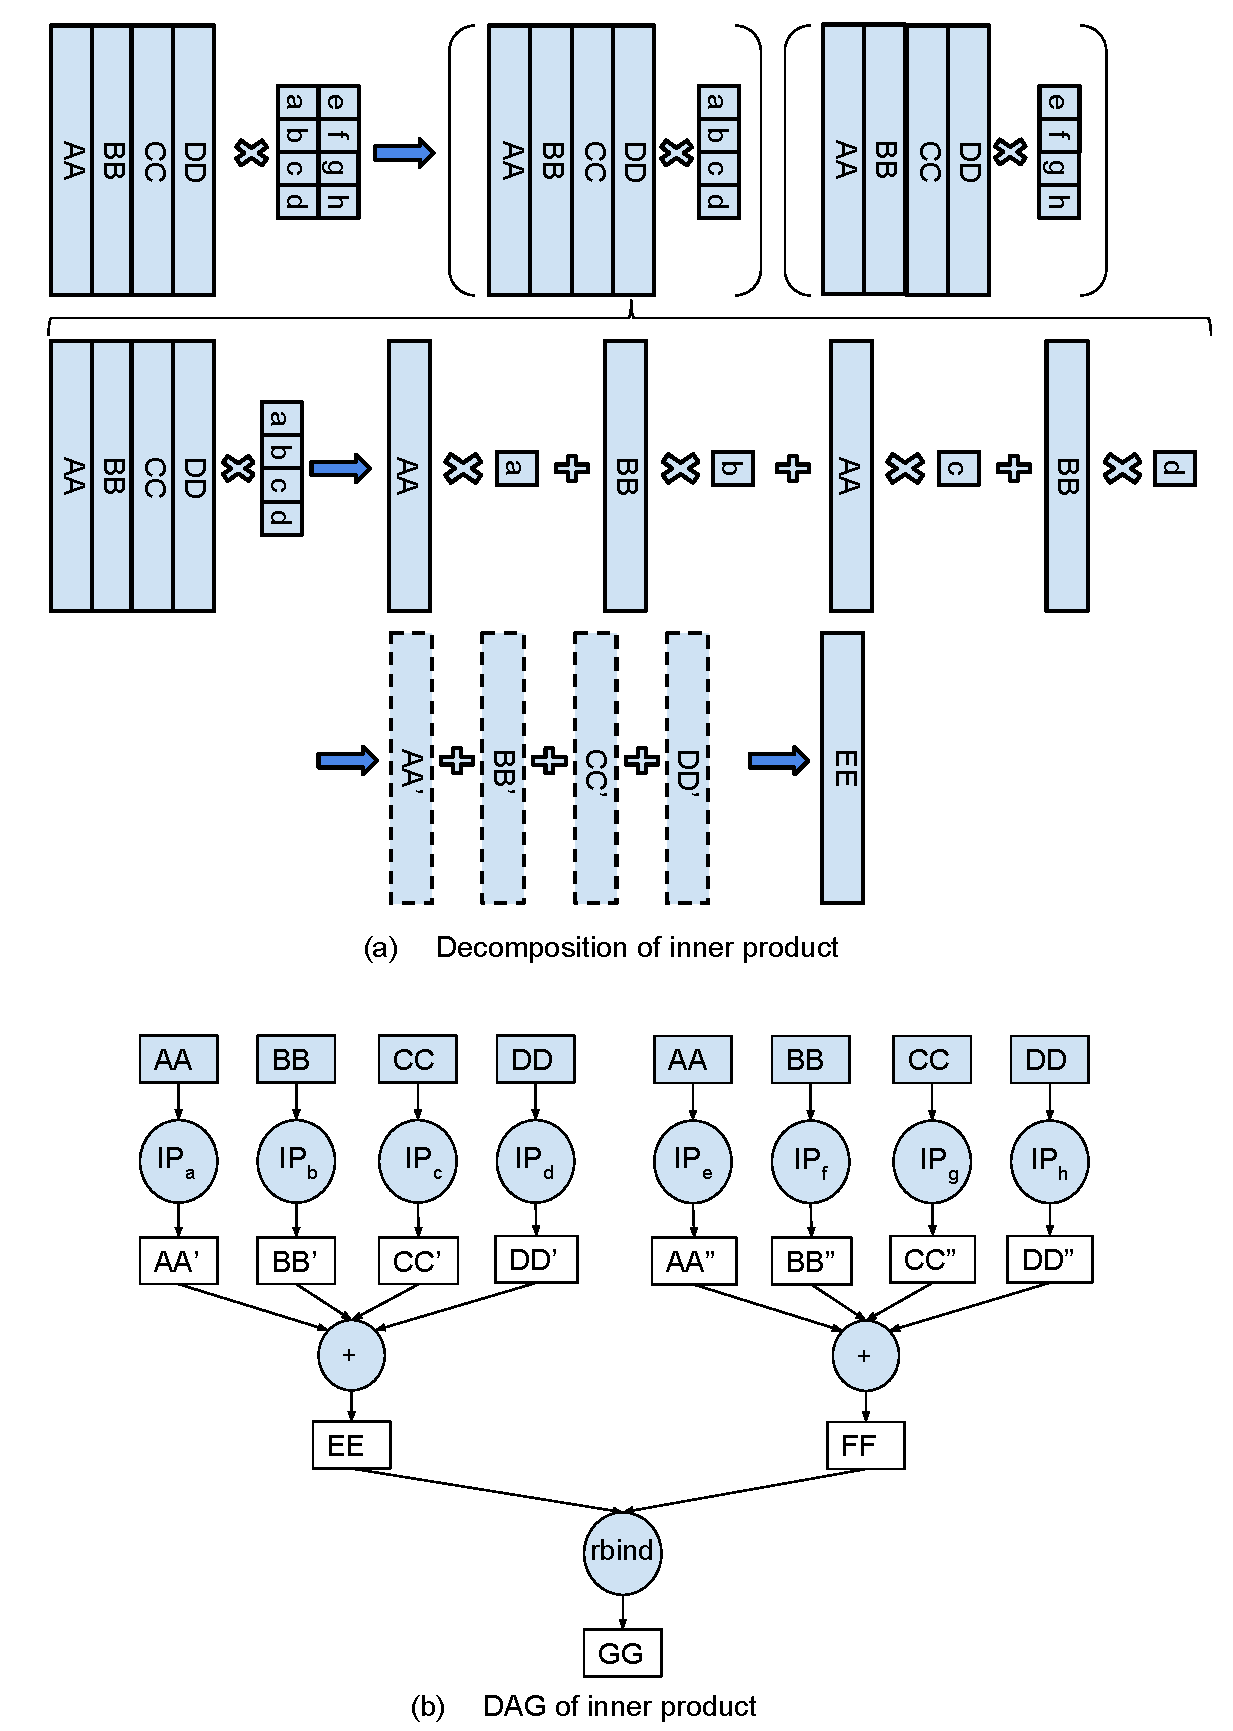
\includegraphics[scale=0.4]{FlashMatrix_figs/inner_prod_tall.pdf}
%\vspace{-5pt}
%\caption{Decomposition inner product on a group of dense matrix.}
%\vspace{-5pt}
%\label{fig:inner_prod}
%\end{figure}

\subsection{Reduce data movement in memory hierarchy}
Although GenOps coupled with VEleFuns achieves efficiency in a single matrix
operation, they alone cannot achieve the overall performance of users' code,
especially when matrices are stored on SSDs. Evaluation of individual matrix
operations results in significant data movement between CPU and SSDs. Even
though the I/O performance of SSDs has advanced to outperform hard drives by
a large factor, they are still an order of magnitude slower than RAM.
To achieve performance, it is essential to reduce data movement between SSDs
and RAM as well as between RAM and CPU when evaluating a sequence
of matrix operations. The first step is to evaluate individual matrix operations
lazily and construct a computation graph. When performing computation in
the computation graph, we take advantage of two-level partitioning on matrices
to reuse data in memory and in CPU cache and reduce data movement in memory
hierarchy.

\subsubsection{Lazy evaluation} \label{sec:lazy_eval}
FlashMatrix allows to evaluate many matrix operations lazily, which includes
all GenOps in Table \ref{tbl:genops} and some utility functions in Table
\ref{tbl:utility}. The lazily evaluated matrices are put together to construct
a directed acyclic graph (DAG) to represent the computation. To help reduce data
movement, FlashMatrix grows a DAG as large as possible.

\begin{figure}
	\centering
	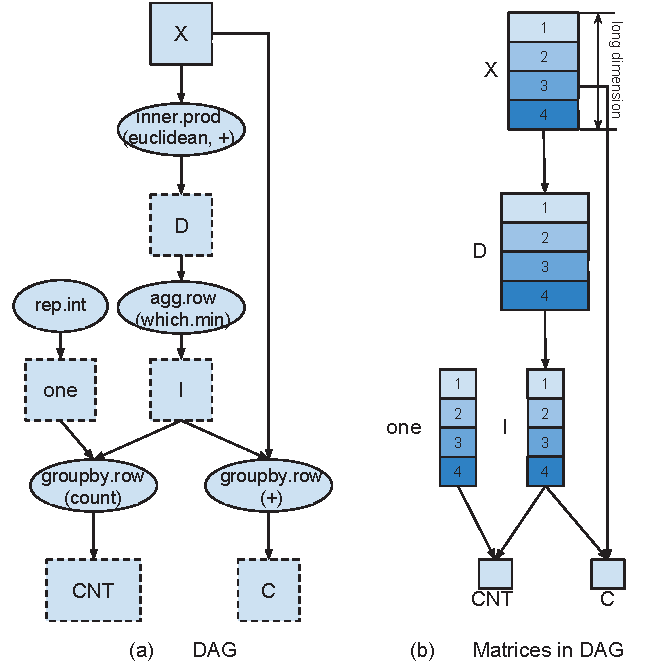
\includegraphics[scale=0.6]{FlashMatrix_figs/KMeans.pdf}
	\caption{A directed acyclic graph of computing an iteration of k-means
	show in Figure \ref{fig:kmeans}.}
	\label{fig:DAG}
\end{figure}

Figure \ref{fig:DAG} (a) shows a DAG for the R code of k-means in Figure
\ref{fig:kmeans}. A DAG comprises a set of matrix nodes (shown as rectangles)
and computation nodes (shown as ellipses). Majority of matrix nodes represent
\textit{virtual matrices}, shown as dashed line rectangles, which only contains
the corresponding matrix operations and input matrices. In the case of k-means,
only the input matrix \textit{X} contains materialized data.
A computation node references to a matrix operation and input matrices and
may contain some immutable computation state, such as scalar variables and
small matrices involved in the matrix computation. 

\textit{Virtual matrices} in a DAG do not need to have
the same shape (Figure \ref{fig:DAG} (b)). All \textit{virtual matrices} in
the internal matrix nodes need to have the same \textit{long dimension} to
simplify evaluation and data flow in matrix materialization. The other dimension
of the internal matrices can vary. The GenOps that generate matrices with
the same \textit{long dimension} as the input matrices include
\textit{fm.sapply} and \textit{fm.mapply}. In addition, FlashMatrix allows
\textit{virtual matrices} of different sizes in both dimensions, such as
matrices \textit{CNT} and \textit{C} (Figure \ref{fig:DAG} (b)), in a DAG.
These \textit{virtual matrices} usually form the edge node of a DAG because
any computation that uses these \textit{virtual matrices} cannot be connected
to the same DAG.  We refer to them as \textit{sink matrices}. The GenOps that
generate \textit{sink matrices} include \textit{fm.agg} and the variants of
\textit{groupby}.

To enable lazy evaluation, all matrices in FlashMatrix are immutable and every
matrix operation generates a new matrix. As such, materialization of
\textit{virtual matrices} always generates the same result. FlashMatrix
garbage collects a matrix when there are no references to it.

\subsubsection{Matrix materialization in the memory hierarchy} \label{sec:materialize}
Lazy evaluation postpones computation in matrix operations, but we eventually
have to materialize some \textit{virtual matrices} to perform actual computation.
When materializing the computation in a DAG, FlashMatrix utilizes the two-level
partitioning in dense matrices to bring data from SSDs to CPU efficiently.

FlashMatrix allows users to materialize any \textit{virtual matrix} in a DAG.
By default, FlashMatrix materializes only \textit{sink matrices} in a DAG to
minimize data written to SSDs because \textit{sink matrices} are small and
are always kept in memory. In the example of k-means (Figure \ref{fig:DAG}),
we materialize the two \textit{sink matrices} together. In some cases,
especially in iterative algorithms,
we need to materialize some non-\textit{sink matrices} in a DAG to avoid
redundant computation and I/O across iterations. In the current implementation,
FlashMatrix allows users to set a flag on the
non-\textit{sink matrices} to inform FlashMatrix to save materialized data
of these matrices to memory or SSDs during computation.

\begin{figure}
	\centering
	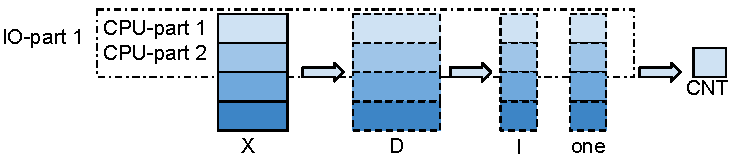
\includegraphics[scale=0.6]{FlashMatrix_figs/materialize.pdf}
	\caption{Materialization of partitions of matrices in a DAG.}
	\label{fig:mater}
\end{figure}

FlashMatrix partitions matrices in a DAG in the \textit{long dimension} and
materializes partitions separately (Figure \ref{fig:mater}). This is realized
because all \textit{virtual matrices} except \textit{sink matrices} in a DAG
share the same \textit{long dimension} size and partition size. As such,
a partition $i$ of a \textit{virtual matrix} only requires data from partitions
$i$ of the parent matrices.
%Owing to
%the storage scheme of in-memory matrices, partitions $i$ of all in-memory
%matrices are stored on the same NUMA node, which minimizes remote memory access.
When materializing a \textit{sink matrix}, each thread first computes partial
aggregation results independently on the partitions of the parent matrix
assigned to the thread. In the end, FlashMatrix merges per-thread partial
aggregation results to construct the \textit{sink matrix}.

%\textit{sink matrices} are usually small and are materialized in memory.
%For example, \textit{agg\_row} on a wide matrix and
%\textit{agg\_col} on a tall matrix outputs a vector. The maximal length of
%the vector is $\sqrt{N}$, where $N$ is the number of elements
%in the input matrix. As such, we can always keep it in memory. For most of machine
%learning and data analysis tasks, the output matrix of the inner product of
%a wide matrix with a tall matrix is usually small and is by default kept
%in memory because the long dimension of these matrices is usually much larger
%than the short dimension in these tasks.

FlashMatrix takes advantage of the two-level partitioning on dense matrices
to reduce data movement between SSDs and CPU. It assigns I/O-level partitions
to a thread as computation tasks for parallelization. We choose a relatively
small partition size to balance the overhead of accessing a partition,
computation skew and memory consumption. A thread further splits
an I/O-level partition into CPU-level partitions at run time and materializes
one CPU-level partition at a time. Materialization of a CPU-level partition
is triggered recursively. As shown in Figure \ref{fig:mater}, materializing
matrix \textit{CNT} triggers materialization of CPU-level partitions of matrices
\textit{I} and \textit{one}, which in turn triggers materialization of
partitions of matrix \textit{D}, and so on. Eventually, it triggers data access
to an I/O-level partition of input matrix \textit{X} from SSDs.
After materializing a CPU-level partition, the thread passes it to the subsequent
operation, instead of materializing the next CPU-level partition in the same matrix.
A CPU-level partition is sufficiently small to fit in the CPU cache so that
the partition still resides in the CPU cache when the subsequent operation consumes
it. This significantly reduces data movement between CPU and memory. In each
thread, all intermediate matrices have only one CPU-level partitions materialized
at any time to reduce CPU cache pollution and thus increase CPU cache hits.
%To reduce CPU cache polution, a CPU-level partition is discarded once it is
%used by all children matrices.

%In a DAG, a matrix may be
%required by multiple GenOps. As such, each matrix always buffers one materialized
%CPU-level partition in each thread to avoid redundant computation.
%\dz{We need to identify transpose of a matrix.}

%FlashMatrix uses a global task scheduler to assign tasks that contains
%computation on I/O-level partitions to threads dynamically for load balancing.
%When the computation involves in-memory matrices, the task scheduler assigns
%tasks to the NUMA node, where the I/O-level partitions of the in-memory matrices
%are stored, to reduce remote memory access.
%However, SSDs require large
%writes to achieve sustainable write throughout and reduce write amplification
%\cite{}. As such, FlashMatrix delays writing the materialized partitions to
%SSDs and merge multiple materialized partitions into a single write because
%the global task scheduler assigns consecutive partitions to threads.

% TODO
%To keep data in CPU cache as long as possible, we reuse the memory buffers
%to reduce the number of memory buffers used in the computation and avoid CPU
%cache polution.

%\subsection{I/O optimizations}

%FlashMatrix maintains per-thread memory buffer pools for accessing I/O-level
%partitions of a matrix on SSDs. These memory buffers have the same size as
%I/O-level partitions, which are in the order of megabytes to maximize I/O
%throughput of an SSD. Because all partitions of a matrix have the same size,
%the memory buffers are reused.
